% Number 660
% CoEM 2D Algebra Units
% Unequal height, numerical methods
% JG

% Watermark
\AddToShipoutPicture*{\BackgroundPic}

\addtocounter {ProbNum} {1}

%\begin{floatingfigure}[r]{.2\textwidth}
%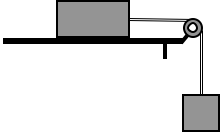
\includegraphics[scale=.6]{/Users/jgates/desktop/latex/pics/halfatwood3}
%\end{floatingfigure}
 
{\bf \Large{\arabic{ProbNum}}} A cannon shoots 9 kg cannonballs off of a 22 meter tall cliff.  The cannon is inclined 17 degrees above the horizontal.  The initial velocity of the cannonballs is ${190~\tfrac{m}{s}}$.

\bigskip
Determine, in two different ways, the speed of the cannonballs when they hit the cliff floor.\paragraph{}
\noindent
\vfill
\vfill

Determine the launch angle that would make the cannonball have the largest possible horizontal range during its flight. You'll have to get creative to solve this equation!
\vfill
%\hfill 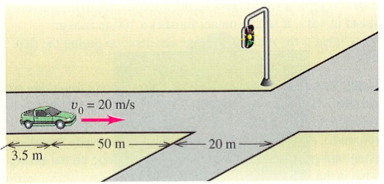
\includegraphics[scale=.85]{/Users/jgates/desktop/latex/pics/redlight.png}
\newpage
